\chapter{Resultaten met de custom  modellen}
\label{ch:resultaten-custom-model}

In ongeveer een kwartier tijd hebben zowel het periodemodel als het themamodel de 845 beelden van Huis van Alijn gelabeld met periodes of thema’s. In die 845 beelden zitten ook de beelden die gebruikt werden voor training en validatie. Het is opmerkelijk om vast te stellen dat ook beelden die als trainingsbeeld ingegeven werden, soms door de modellen fout geclassificeerd worden.

In dit hoofdstuk worden afzonderlijk de resultaten van beide modellen besproken. Tot slot zal net als in hoofdstuk \ref{ch:resultaten-ingebouwd-model} suggesties gedaan worden voor de toepassing van de modellen in de praktijk.
    
Net zoals het ingebouwde model uit het vorige hoofdstuk, geven de custom modellen meerdere tags per foto. Omdat een foto slechts ingedeeld kan worden in één thema, houden we enkel rekening met de tag die de hoogste waarschijnlijkheiddscore gekregen heeft. 

\section{Themamodel}
\label{sec:themamodel}

Het Themamodel heeft 845 beelden geanalyseerd en geclassificeerd. 753 beelden (89\%) werden correct geclassificeerd.  De waarschijnlijkheidsscore van de tags bevond zich tussen 100\% en 39\% en had een gemiddelde van 94,6\%. De gemiddelde rappel voor de vijf thema’s is 90\%, terwijl de gemiddelde precisie een waarde van 86\% heeft.

\begin{table}
	\centering
     \renewcommand\arraystretch{1.2}
    \begin{tabular}{l|ccc|rrr}
        \toprule
         & true positives  & false negatives & false positives & rappel & precisie & \textit{F}-score \\
        \midrule
        geboorte & 81 & 15 & 50 & 84,4\% & 61,8\% & 71,4\% \\
        huwelijk & 346 & 54 & 6 & 86,5\% & 98,3\% & 92\% \\
        Sint & 93 & 4 & 1 & 95,9\% & 98,9\% & 97,4\% \\
        speelgoed & 88 & 13 & 21 & 87,1\% & 80,7\% & 83,8\% \\
        vakantie & 145 & 6 & 14 & 96\% & 91,2\% & 93,6\% \\
        \midrule
        gemiddelde & 150,6 & 18,4 & 18,4 & 90\% & 86,2\% & 87,6\% \\
        \bottomrule
    \end{tabular}
    \caption{De resultaten (rappel, precisie en \textit{F}-score) van het Themamodel op de volledige dataset van Huis van Alijn.}
    \label{tab:resultaten-themamodel}
\end{table}

Qua thema’s wordt de hoogste \textit{F}-score behaald bij het thema Sinterklaas (97\%). Dit thema haalde in hoofstuk \ref{ch:resultaten-ingebouwd-model} nog de slechtste resultaten, maar heeft in deze test de grootste precisie en de tweede grootste rappel. Dit is te verklaren doordat de foto’s sterk op elkaar lijken. Op iedere foto staat een oudere man met baard en mijter, vergezeld door een of meerdere kinderen die met de oude man op de foto poseren. Opvallend is ook de sterke score van de vakantiefoto’s (\textit{F}-score van 94\%), terwijl deze foto’s juist gekenmerkt worden door een grote variëteit (strandfoto’s, kampeerfoto’s, citytrips, wintersport,...).

De slechtste score wordt behaald met de geboortefoto’s. Vooral de precisie voor deze foto’s zijn ondermaats (62\%). Dit thema heeft 50 false positives\footnote{Dit zijn 50 foto's die foutief het label geboorte kregen.}. Veel huwelijksfoto’s (54 false negatives\footnote{~Dit zijn 54 huwelijksfoto's die niet als huwelijksfoto herkend werden.}) worden namelijk als geboortefoto herkend.  Net als in vorig hoofdstuk scoren de speelgoedfoto’s ook niet zo goed. Zowel de precisie als de rappel zijn lager dan het gemiddelde.

Sommige lagere scores zijn te wijten aan de vaag afgebakende thema’s door het museum. Sommige foto’s die door het museum ingedeeld werden in het thema speelgoed zijn  foto’s van kinderen met een stuk speelgoed op vakantie, terwijl er ook vakantiefoto’s zijn waar kinderen met speelgoed op poseren. Dit verklaart waarom het model zeven speelgoedfoto’s classificeert als vakantiefoto’s en vier vakantiefoto’s als speelgoedfoto’s. Het model heeft het ook moeilijk om poppen van baby’s te onderscheiden. Negen geboortefoto’s werden door het model ingedeeld in het thema speelgoed, terwijl zes speelgoedfoto’s als geboortefoto’s beschouwd werden (zie confusion matrix \ref{tab:confusion-matrix-themamodel}).

Net zoals in vorig hoofdstuk werd geanalyseerd of het model slecht scoort op foto’s uit bepaalde decennia. Dit lijkt niet het geval te zijn. Foto’s uit de jaren 60 (en 50) hebben een grotere foutenmarge, maar dit valt weer te verklaren door de grote hoeveelheid huwelijksfoto’s uit deze periode.

\begin{table}
    \centering
    \renewcommand\arraystretch{1.2}
    \settowidth\rotheadsize{\theadfont Feitelijk thema}   
    \begin{tabular}{@{} cc | cccccc}
        \toprule
        &  & & \multicolumn{5}{c}{\textbf{Voorspeld thema}}  \\
        &  & & geboorte & huwelijk & sint & speelgoed &  vakantie  \\
        \midrule
        \multirow{5}{*}[1ex]{\rothead {\textbf{Feitelijk thema}}}
        & geboorte   &  &  \cellcolor{hgpink}81 & 3 & 1 & 9 & 2 \\
        & huwelijk  &   & 43 & \cellcolor{hgpink}346 & 0 & 6 & 5 \\
        & sint  &   & 1 & 1 & \cellcolor{hgpink}93 & 2 & 0 \\
        & speelgoed  &  & 6 & 0 & 0 & \cellcolor{hgpink}88 & 7 \\
        & vakantie & & 0 & 2 & 0 & 4 & \cellcolor{hgpink}145 \\
        \bottomrule
    \end{tabular}
    \caption{Confusion matrix voor het Themamodel}
    \label{tab:confusion-matrix-themamodel}
\end{table}

\section{Periodemodel}
\label{sec:periodemodel}

Ook het Periodemodel heeft 845 beelden geanalyseerd en geclassificeerd. Omdat van 42 beelden de periode niet gekend was door het museum en we dus niet konden nagaan of het model ze juist geclassificeerd heeft, werden deze beelden niet meegerekend bij de beoordeling van de resultaten. 

Het model had 460 beelden (57\%) correct geclassificeerd. De waarschijnlijkheidsscore van de tags bevond zich tussen 94\% en 20\% en had een gemiddelde van slechts 55\%. Dit kan betekenen dat het model ofwel te weinig trainingsbeelden had om de verschillende concepten te kunnen onderscheiden, of dat de taak te moeilijk is voor een CV API. De gemiddelde rappel voor de tien periodes is maar 57\%, terwijl de gemiddelde precisie een waarde van 62\% heeft.

\begin{table}
	\centering
    \renewcommand\arraystretch{1.2}
    \begin{tabular}{l|ccc|rrr}
        \toprule
        & true positives  & false negatives & false positives & rappel & precisie & \textit{F}-score \\ 
        \midrule
        00s & 3 & 6 & 0 & 33,3\% & 100\% & 50\% \\ 
        10s & 13 & 3 & 8 &  81,3\% & 61,9\% & 70,3\% \\ 
        20s & 14 & 18 & 15 & 43,8\% & 48,3\% & 45,9\% \\ 
        30s & 34 & 20 & 45  & 63\% & 43\% & 51,1\% \\ 
        40s & 40 & 21 & 70  & 65,6\% & 36,4\% & 46,8\% \\ 
        50s & 110 & 99 & 71  & 52,6\% & 60,8\% & 56,4\% \\ 
        60s & 120 & 106 & 56  & 53,1\% & 68,2\% & 59,7\% \\ 
        70s & 73 & 41 & 51  & 64\% & 58,9\% & 61,3\% \\ 
        80s & 43 & 18 & 24  & 70,5\% & 64,2\% & 67,2\% \\ 
        90s & 10 & 11 & 3  & 47,6\% & 77\% & 58,8\% \\ 
        \midrule
        gemiddelde & 46 & 34,3 & 34,3  & 57,5\% & 61,9\% & 56,7\% \\ 
        \bottomrule
    \end{tabular} 
    \caption{De resultaten (rappel, precisie en \textit{F}-score) van het Periodemodel op de volledige dataset van Huis van Alijn.}
    \label{tab:resultaten-periodemodel}
\end{table}

De hoogste F-score wordt behaald bij foto’s van de jaren 10 (70\%). Dit is nochtans een van de periodes met het laagst aantal trainingsbeelden (8 beelden). Vooral de rappel voor deze periode is erg goed (81\%). Ook de 80s scoren goed met een F-score van 67\%. Over het algemeen scoren de periodes vanaf de jaren 60 het best, waarbij de jaren 10 de uitzondering is. Misschien zijn zwart-wit foto’s uit de jaren 20 tot en met 60 vergelijkbaar qua kleur?

De slechtste scores worden behaald met foto’s uit de jaren 20 en 40, met een respectievelijke F-score van 46\% en 47\%. Bij de jaren 40 is de rappel goed (66\%), maar is de precisie erg laag (36\%). Het heeft namelijk 70 false positives. Dit komt doordat veel foto’s uit de jaren 50 (43 foto’s), en in mindere mate jaren 60 (13 foto’s) en 30 (9 foto’s), herkend wordt als een foto uit de jaren 40. Als het model fout is, dan vergist het zich meestal met de omliggende periodes (zie confustion matrix \ref{tab:confusion-matrix-periodemodel}).

\begin{table}
    \centering
    \renewcommand\arraystretch{1.2}
    \settowidth\rotheadsize{\theadfont Feitelijk thema}
    
    \begin{tabular}{@{} cc | ccccccccccc}
        \toprule
        &  & & \multicolumn{10}{c}{\textbf{Voorspelde periode}}  \\
        &  & & 00s & 10s & 20s & 30s & 40s & 50s & 60s & 70s & 80s & 90s \\
        \midrule
        \multirow{10}{*}[1ex]{\rothead {\textbf{Feitelijke periode}}}
        & 00s   &  & \cellcolor{hgpink}3 & 2 & 1 & 0 & \cellcolor{hgpink}3 & 0 & 0 & 0 & 0 & 0 \\
        & 10s  &   & 0 & \cellcolor{hgpink}13 & 1 & 1 & 1 & 0 & 0 & 0 & 0 & 0 \\
        & 20s  &   & 0 & 2 & \cellcolor{hgpink}14 & \cellcolor{hgpink}12 & 0 & 3 & 0 & 0 & 0 & 0 \\
        & 30s  &  & 0 & 0 & 4 & \cellcolor{hgpink}34 & 9 & 4 & 3 & 0 & 0 & 0 \\
        & 40s & & 0 & 1 & 2 & 4 & \cellcolor{hgpink}40 & 13 & 0 & 0 & 0 & 0 \\
        & 50s   &  & 0 & 3 & 3 & 15 & 43 & \cellcolor{hgpink}110 & 32 & 3 &0 & 0 \\
        & 60s  &   & 0 & 0 & 3 & 8 & 13 & 42 & \cellcolor{hgpink}120 & 31 & 9 & 0 \\
        & 70s  &   & 0 & 0 & 1 & 3 & 0 & 9 & 19 & \cellcolor{hgpink}73 & 8 & 1 \\
        & 80s  &  & 0 & 0 & 0 & 0 & 0 & 0 & 2 & 14 & \cellcolor{hgpink}43 & 2 \\
        & 90s & & 0 & 0 & 0 & 1 & 0 & 0 & 0 & 3 & \cellcolor{hgpink}7 & \cellcolor{hgpink}10 \\
        \bottomrule
    \end{tabular}
    \caption{Confusion matrix voor het Periodemodel}
    \label{tab:confusion-matrix-periodemodel}
\end{table}

Twee periodes behalen een lage rappel, maar een erg hoge precisie. Foto’s uit de jaren 00 hebben een rappel van slechts 33\%, maar een precisie van 100\%; voor de jaren 90 gaat het om een rappel van 48\% en een precisie van 77\%. Deze periodes scoorden tevens minder goed in de validatieset en behoren tot de groep met het minst aantal trainingsbeelden (respectievelijk vier en tien beelden). 

\section{Toepassen in de praktijk?}
\label{sec:custom-toepassen-praktijk}
Het Periodemodel is niet voldoende performant om in de praktijk toe te passen. De foutenpercentage is te hoog en de waarschijnlijkheidsscores zijn te laag om goede conclusies te kunnen trekken. In deze sectie wordt daarom enkel gefocust op het Themamodel.

Het is moeilijker dan in \ref{sec:ingebouwd-toepassen-praktijk} om duidelijke conclusies te trekken omdat we slechts 845 resultaten hebben om te beoordelen. Uit de resultaten lijkt dat een CV API vooral goed te trainen is op beelden die een duidelijke weergave en thematiek hebben, zoals de Sinterklaasfoto’s.

Wat betreft waarschijnlijkheidsscores en drempelwaarden zijn er twee strategieën die gevolgd kunnen worden: 
\begin{enumerate}
        \item instellen van een drempelwaarde;
        \item rekening houden met de waarschijnlijkheidsscore van de concept met de tweede hoogste score.
\end{enumerate}

\subsection{Instellen van een drempelwaarde}
Zoals reeds vermeld is de gemiddelde waarschijnlijkheidsscore 94,6\% voor zowel juist als foutief geklasseerde foto’s. De gemiddelde waarschijnlijkheidsscore voor de juiste classificaties ligt echter hoger (97\%), terwijl die voor de foute lager ligt (77\%). De mediaan\footnote{De mediaan is het midden van een verzameling van gegevens. 50\% heeft bijgevolg een waarde lager dan de mediaan; 50\% dan weer een waarde hoger dan de mediaan.} is respectievelijk 100\% en 80\%. Het is hierbij dus mogelijk om een drempelwaarde in te stellen. In tabel worden enkele potentiële drempelwaarden voorgesteld.  

\begin{figure}
	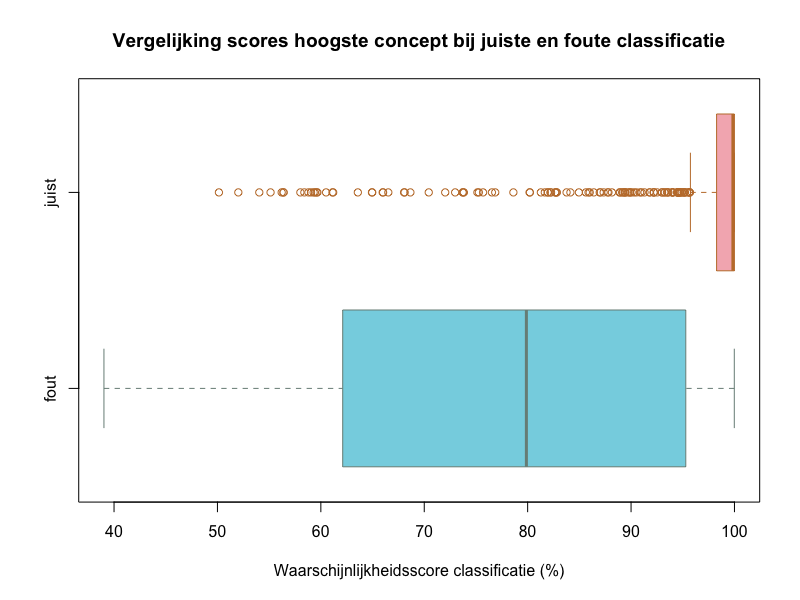
\includegraphics[width=\textwidth]
	{boxplot_hoogste_concept.png}
	\caption[Vergelijking van de waarschijnlijkheidsscores van de juiste en foute classicaties van het custom model]{Twee boxplots die de waarschijnlijkheidsscores vergelijken van het Periodemodel bij juiste en foute classificatie. In tegenstelling tot in figuur \ref{fig:boxplot-clarifai} is er geen overlap tussen de interkwartielafstand van de foute classificaties en de boxplot van de juiste classificaties.}
	\label{fig:boxplot-tag1}
\end{figure}

%TODO tabel invoegen

\subsection{Rekening houden met de waarschijnlijkheidsscore van de tweede tag}
Anderzijds kan er ook gekeken worden naar de waarschijnlijkheidsscore van het tweede hoogste concept dat door het model gegeven wordt. Als het model een foto correct geclassificeerd heeft, dan krijgt het tweede concept in 64\% van de gevallen een waarschijnlijkheiddscore van (afgerond) 0\%.\footnote{De mediaan is bijgevolg 0\%} Wanneer het model een foto fout geclassificeerd heeft, dan ligt de mediaan van de waarschijlijkheidsscore voor het tweede concept op 17\% en het gemiddelde op 19\%. In 50\% van de gevallen heeft het tweede concept dan een waarschijnlijkheidsscore hoger dan 17\%. Door de tags te weerhouden waarvan het tweede concept een te hoge score heeft, kunnen eveneens fouten vermeden worden. In tabel worden hiervoor ook enkele voorstellen gedaan.

\begin{figure}
	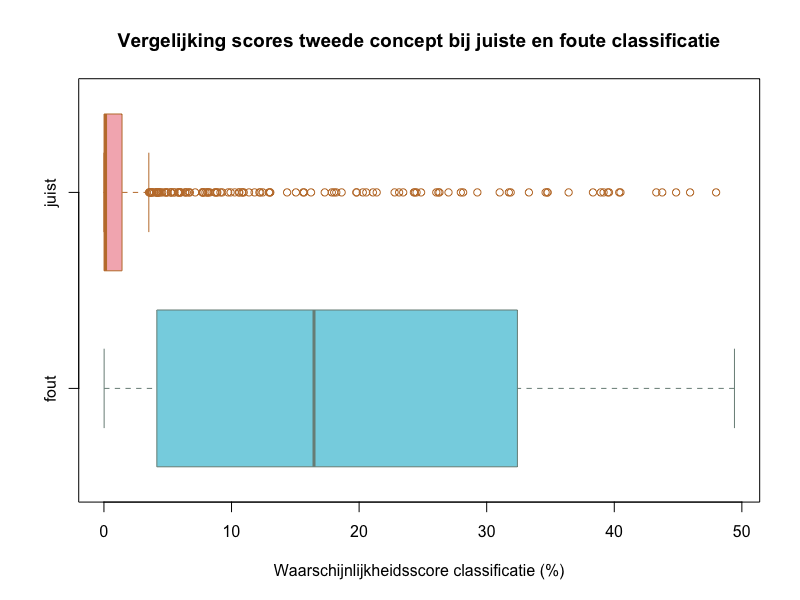
\includegraphics[width=\textwidth]
	{boxplot_tweede_concept.png}
	\caption[Vergelijking van de waarschijnlijkheidsscores van de juiste en foute classicaties van het custom model]{Twee boxplots die de waarschijnlijkheidsscores vergelijken van het tweede concept van het Periodemodel bij juiste en foute classificatie. Net als in figuur \ref{fig:boxplot-tag1} is er geen overlap tussen de interkwartielafstand van de boxplot van de foute classificatie en de boxplot van de juiste classificatie.}
	\label{fig:boxplot-tag2}
\end{figure}

%TODO tabel invoegen

